\documentclass[bsc]{abdnthesis}
\usepackage[T1]{fontenc}
\usepackage{url}
\usepackage{hyperref}

\graphicspath{ {./img/} }

\author{Anthony Sergio Chapman}
\Supervisor{\\Dr Steve Turner \\ Dr Lorna Aucott \\  Dr Wei Pang}
\title{9-Month Assessment Report}
\school{Department of Applied Health Sciences}
\date{2015}

\begin{document}
\maketitle
\makedeclaration


\begin{abstract}
There is a large body of evidence linking reduced birth weight and increased risk for non-communicable diseases (NCD) such as type II diabetes and asthma, and this implicates factors driving fetal growth in NCD aetiology. We are exploring the potential for a computing approaches to relating repeated measurements of fetal size during a pregnancy to post natal outcomes using routinely acquired data for the population of Grampian.

Routinely acquired data will be linked and approvals sought.  The current approach is as follows: using multiple imputation, we will address missing data. After the data are ready for processing, clustering will be used to group the data into subsets with similar traits. Each subset will be statistically analysed and outcomes will be derived by their antenatal measurements. The outcomes of interest are NCD which can be determined in children and include obesity, asthma, eczema, epilepsy and type I diabetes.
\end{abstract}

\begin{acknowledgements}
  Thank god for tea!
\end{acknowledgements}

\tableofcontents
%\listoftables
%\listoffigures

\clearpage
\setcounter{page}{1}

\chapter{Introduction}
This chapter introduces the 9 month report, presents the research questions and gives a quick overview of some of the background and motivations for this PhD. 

\section{Early Assessment} % (fold)
\label{sec:early_assessment}
I would like to mention that I started this PhD in mid-December but wish to take part in the 9-month assessment at the same time as everyone else. One of the main reasons for this is that I wish to go to the Summer Symposium and present my work to and with everyone else. 

My progress up to date has been efficient and I have identified key issues, problems and possible solutions to my research questions very early on. I will talk about these in more details throughout this report. I will also mention our communications with other universities whom are interested in similar research and the possibility of collaborative work.
% section early_assessment (end)
\section{Background} % (fold)
\label{sec:background}
There is a large body of evidence linking reduced birth weight and increased risk for non-communicable diseases (NCD) such as type II diabetes and asthma\cite{ turner1, turner2, turner3, generation-r1, generation-r2}, this implicates factors driving fetal growth in NCD aetiology. There is an emerging literature describing associations between fetal size and growth and NCD. The goal of this project is to find efficient computational approaches to solve such problems in a greater scale. 

We are exploring the possibility for a computational approach to relating repeated measurements of fetal size during a pregnancy to post natal outcomes using routinely acquired data for the population of Grampian. If successful, our approach has the potential to be used nation wide or even internationally. 

Research within this field is being carried out throughout the world. Generation R projects have included asthma origins \cite{ generation-r1} as well as their symptoms in early childhood \cite{ generation-r2}. Other researchers from Italy and Russia are also looking at fetal growth trajectories \cite{luccia1, luccia2, luccia3, luccia4}. 

Issues we will need to address include missingness of data, comparison between different anthropometric measurements for the same individual and the anticipation that different growth trajectories will be associate with the same increased risk for NCS.  
% section background (end)
\section{Research Questions} % (fold)
\label{sec:research_questions}
Our current research can be split into two sections which are as follows:
\subsection{Methodological} % (fold)
\label{sub:methodological}
Our first question relates to the analysis of partially complete data. When there are large amounts of missing values in a dataset, can we still perform efficient data analysis. We consider this using imputation techniques. Thus, our hypothesis is: Data analysis is possible and efficient using appropriate imputation techniques on datasets with partially complete records.

How accurate is gestational assessment. 
% subsection methodological (end)
\subsection{Epidemiological} % (fold)
\label{sub:epidemiological}
Using cluster analysis, one can gather complex relationships between fields in datasets. In this manner we are going to find the relationships between fetal and maternal characteristics to NCD in children and adults. Thus, our question is: What are the relationships between the measurements and NCD. One early hypothesis is that steady growth will be associated with a decreased risk for postnatal NCD, another hypothesis would then be that change of growth will increase the risk for postnatal NCD. 
% subsection epidemiological (end)
% section research_questions (end)


\chapter{Key Issues}
Our group has acquired a number of sample datasets, these datasets represent the actual data to be analysed. By analysing and experimenting with these datasets we have been able to identify key issues and ideas which are critical for the success of this project.
\section{Missingness} % (fold)
\label{sec:missingness}
At first glance, we noticed that the sample datasets have vast amounts of data missing. If the sample data we have truly represents the real data, missingness is an issue that will have to be resolved. 

One of the biggest problems missingness induces, is that of reliability or confidence in any analysis results. For example, 30\% of population would be enough to confidently state anything about the population as a result of analysis the 30\%, but what if only 15\% of that 30\% is complete? That leaves us with only 4.5\% of the population, which would not be enough to justify any statement about the population. 

We can not, however, disregard the data with partial missingness. Information, important or not, can still be gathered from missing or partially missing data. 

Imputation is the process of replacing missing data with some values\cite{ imp}. There exist a full range of imputation techniques from simple default value substitution (ie replacing all missing values with some values)\cite{ imp-default}, slightly more clever ways such as mean values substitution \cite{ imp-mean}(similar to default value substitution except here the values may change according to the dataset), to very complicated imputation which works by calculating probabilities of values according to the know ones\cite{ imp-mice, imp-mi}. 
% section missingness (end)
\section{Clustering and Cluster Validation} % (fold)
\label{sec:clustering_and_cluster_validation}
We have been looking at ways to incorporate clustering techniques for real world data analysis.  Clustering is a way of grouping data into different sections, called clusters, these clustering will contain data points which are most similar to each other \cite{ cluster}. The way a computer considers data points to be similar is problem dependant. By grouping the data into different clusters, we are able to analyse patterns, trends or relationships in datasets. 

We hope to find that by clustering maternity data, antenatal behaviours and trends will be made clear. For example, we might find that a certain cluster who's records all have similar growth rates also have a some NCD, implying relationships. This approach eliminates any bias statistical regression modelling might induce by specifically looking for a certain relationship. Here, the algorithm looks for any relationships without focusing on any specific one. 

By letting the algorithm analyse the data without focusing on specific relationships between trends and outcomes, we hope to find interesting and possibly unexpected results, moreover, by not specifically looking for such results, the results will be more reliable. 

Cluster validation is used to evaluate cluster outcomes\cite{ cluster-val}. This is useful in order to assess the validity of a clustering, it can then be used to compare clustering algorithms or even different datasets against each other. 

Using clustering and cluster validation techniques, we will be able to assess the efficiency and other effects imputation will cause when you create artificially complete datasets from partially missing ones. We will also be able to evaluate the efficiency as well as the correctness or confidence in any outcomes we get by clustering data. 

If we are going to use clustering techniques to discover information from the data, cluster validation will be used to test the efficiency as well as the correctness of the outcomes we discover. It will also be useful when handling missing data, we will be able to used cluster validation to check the effects on running any imputation technique to datasets.  
% section clustering_and_cluster_validation (end)
\section{Growth Trajectories} % (fold)
\label{sec:growth_trajectories}
From the sample data, we can see that the measurements are consist of some volume/size measurements (trimesters and weight at 5 years) and some categorical measurements (maternal data, smoking, previous asthma economics), as shown in Figure~\ref{sample_data}. In order to analyse the growth characteristics and determine any relationships to diseases and disorder, a growth trajectory needs to be defined. 

\begin{figure}[h]
  \centering
    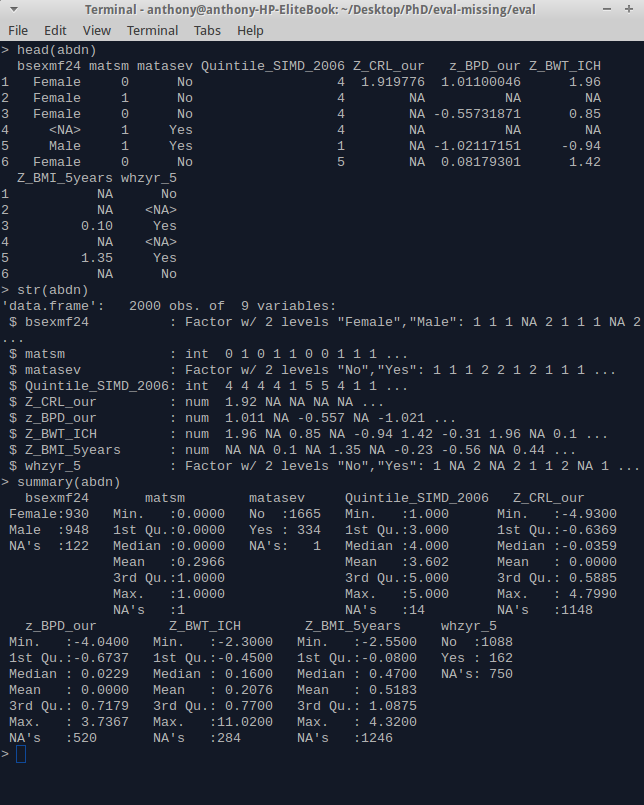
\includegraphics[width=0.4\textwidth]{sample_data}
  \caption{Summary of one of the sample datasets.}
  \label{sample_data}
\end{figure}

The datasets consist of growth measurements, which alone are not enough to describe a growth trajectories that could represent the whole data. What we need is a model to describe a growth trajectory in terms of the growth measurements and produces a growth curve or formula.

Using only the growth measurements would not be enough. As already mentioned, we also have growth characteristics such as whether the mother smoked. These categorical datum have to be taken into account also. 

Mixed modelling is a way of statistically modelling data with mixed (numerical and categorical) data. It will be able to take into account categorical data and use it to change any growth trajectory to make it more realistic. This is no to be confused with mixed effects modelling which uses fixed and random effect equations for statistical modelling. 
% section growth_trajectories (end)


\chapter{Literature Review}
This chapter covers some of the current work which inspire our current ideas, some topics related to the research questions and some of the methods we believe will help solve the questions.
\section{Imputation} % (fold)
\label{sec:imputation}
Imputation is the process of replacing missing fields with values\cite{ imp}. There is a huge array of imputation techniques ranging from straight forward default value imputation \cite{ imp-default}, to mean-value imputation \cite{ imp-mean} or even imputation by equations \cite{imp-mi, imp-mice}. 

Default value imputation techniques are not appropriate as I believe they are too biased. By choosing to replace all missing fields with one value, the data is shifted into a direction which might (with high probability) jeopardise any underlying relationships within the dataset. Similarly, mean value imputation does not consider enough of the dataset to produce reliable imputations. It only looks at one field at a time and does not consider the relationship between different fields in each record. This could also negatively affect the results of any analysis carried out. 

Multiple Imputation by Chained Equations (MICE) \cite{imp-mice} considers both the relationship between the fields of each record and the behaviour of all the other records in the dataset. I have chosen to use MICE to impute my data, given that all data behaves differently, a method for evaluating the efficiency of MICE on my datasets will have to be created. 
% section imputation (end)
\section{Clustering} % (fold)
\label{sec:clustering}
R, the statistical program \cite{R}, has some very good clustering packages available \cite{ cran} for the public to use. The most widely used ones are "cluster" \cite{clust-cluster}, "cclust" \cite{ clust-cclust}, "fclust" \cite{ clust-fclust} and "mclust" \cite{ clust-mclust}. They can all perform similar clustering techniques, they differ in terms of efficiency and the type of data they can cluster efficiently. 

The package "mclust" is comfortable performing model-based clustering using mixture models. This is useful when the datasets follow a multi model tier structure. Although powerful, our data is not complicated enough to justify using this package as other packages would perform the same clustering without over-complicating the process. This leads to a more efficient (in terms of speed in this case) process. 

Similarly, "fclust" works well with fuzzy data were the clustering can be ambiguous. It can cluster data with levels of certainty where other clustering techniques have a binary approach, it is either in a cluster or not. Again, our data is not so complex to need such techniques. 

The main choice lies between "cluster" and "cclust", "cluster" is the original package and has more online support, whereas "cclust" has a better indexing system which is better for finding the optimal number of clusters a dataset needs. 

Tests and evaluations will have to be carried out to see which should be used. My prediction for the most efficient way to do this would be; use "cclust" for finding the optimal number of clusters and then, using this number, we perform a clustering using the package "cluster". It will need to be tested but by using both their strengths, I might have the best clustering available
% section clustering (end)
\section{Growth vs Asthma} % (fold)
\label{sec:growth_vs_asthma}
Our group  have related fetal measurements to postnatal outcomes in childhood which include asthma and eczema in a local population \cite{turner1, turner2, turner3} and also from Saudi Arabia \cite{ saudi}.  Our work and a systematic review of the literature demonstrates that small absolute fetal size and either accelerating or faltering fetal growth are all associated with adverse outcomes. 

The methods used are simple statistical regressions, with confidence intervals to indicate how valid the analysis is. Our new ideas consist of efficient computational approaches to solve such problems in a greater scale as well as with greater confidence in the findings.

Our proposed approach differs as the biggest problems in using statistical models for analysis is that regardless of the confidence level, they are wrong. The analyst's job is to find the least wrong. Our approach will be less probabilistic and thus give the outcomes more confidence. 
% section growth_vs_asthma (end)

% \section{European Thesis} % (fold)
% \label{sec:european_thesis}
% I analysis the structure of European theses \cite{generation-r1, generation-r2} vs the structure of British theses 
% % section european_thesis (end)

\section{Regression Modelling} % (fold)
\label{sec:regression_modelling}
An important aspect of this project is to choose an appropriate way to model fetal growth from the maternity data. R has many regression modelling packages, the ones considered for this project are a linear modelling package (lm \cite{lm}), a mixed effects modelling modelling package (lme4 \cite{lme4}) and a latent growth modelling package (lavaan \cite{lavaan}). 

Each package treats the data slightly differently, currently we are focusing on addressing the issue of missingness and thus are using a simple linear model under the package "lm" to evaluate imputed datasets. 

Mixed effects modelling techniques are not required at this stage of the project although they might be useful if we want to find complex inter-field relationships, ie relationships between fields, whilst simultaneously performing a regression model. 

We also have an idea, its at early stages yet, for using latent growth modelling to create a fetal growth trajectory. Currently, the data contains only fetal size variables and maternal details, not any actual growth measurements. Thus we can not create a regression model on growth itself, we can only model size in terms of the other variables. Using latent growth modelling we can eliminate that as we can take growth to be our latent variable. 
% section regression_modelling (end)

% \chapter{Transferable Skills}

\chapter{Progress}
\section{Presentation Skills} % (fold)
\label{sec:presentation_skills}
At the beginning of this PhD I attended two courses in presentation skills and one in good clinical practice (GCP). The presentation skills courses, offered by the university, were very educational. The first focused on key factors for giving a memorable, entertaining and educational presentation, it included some interesting techniques to keep the audience focused. The second concentrated on how to use ones voice when presenting work, it included basic voice training, warming techniques and some practise. 
% section presentation_skills (end)
\section{Approvals and training} % (fold)
\label{sec:approvals_and_training}
Approvals for gaining access to the routinely acquired maternity data for analysis have been submitted. Coursed required to acquire the data have been identified and have been taken (GCP) or registration has been completed and we are waiting to do the courses (information governance online course).
% section approvals_and_training (end)
\section{Italian Partners} % (fold)
\label{sec:italian_partners}
At early stages of this project, we became acquainted with a Lucia Vaira, a second year PhD student at the University of Salento, Italy. Vaira's research is in fetal growth curves and a unified method for global fetal growth analysis \cite{ luccia1, luccia2, luccia3}. 

After brief talks on our relevant fields of research, we discussed the possibility of collaborating together. We are currently writing a joint research paper focusing on fetal growth regression modelling. We have not yet identified a conference to present the paper and the paper is near completion. 
% section italian_partners (end)
\section{ACERO Symposium} % (fold)
\label{sec:acero_symposium}
The Aberdeen Centre for Energy Regulation and Obesity (ACERO) held their annual symposium at the Rowett Institute of Nutrition and Health in Aberdeen\cite{ acero}. I volunteered to give a short presentation on how to evaluate artificially completing datasets. 

It was a great experience, nerve-racking but good practise for future presentations. The questions at the end raised good points and it gave me a chase to experience public speaking. The courses taken on presentation skills earlier in the year certainly came to good use. 

One this to work on from this experience is to finish presentations on harder notes. We need to reinforce to the audience what exactly they should take away from the presentation. Overall, it was a success. 
% section acero_symposium (end)
\section{FARR International} % (fold)
\label{sec:farr_international}
In August 2015 the Farr Institute shall be hosting their first International Conference in St Andrews\cite{ farr}. I have submitted an abstract and await their decision on whether I shall be presenting there. It will be great experience regardless on whether I present or not as it will let me know meet other researchers from around the world. 
% section farr_international (end)
\section{FARR PhD Symposium} % (fold)
\label{sec:farr_phd}
The Farr Institute PhD Symposium will be held on 9th June 2015 in Manchester\cite{ farr-phd} and is open to all PhD students associated with the Farr Institute. All PhD students who wish to go to the symposium are required to submit an abstract, we will then be chosen to either give a talk or present a poster. 

Again, this is a great chance to meet other PhD students from across the United Kingdom. If chosen for a presentation, I will talk about missingness and my plan on how I'm going to carry out the rest of this PhD.
% section farr_phd (end)


\chapter{Future Plans}
I will do stuffs.
\section{The next steps:} % (fold)
\label{sec:immediate_things_to_do_}
% section immediate_things_to_do_ (end)Immediate things to do:
\begin{itemize}
	\item FARR PhD symposium academic poster \\ - On the 10th June 2015, I will be attending the annual FARR PhD symposium where I have been asked to create an academic poster and present it at the symposium. The poster will be based on our efforts to create artificially complete data and some results showing that the new data is a good representation of the truth.
	\item Finish and submit PAC application for approval \\ - The sooner this application is submitted, the sooner we are able to gain access to Aberdeen's maternity records. I am in the process of completing this lengthy application in order to send it soon. Once this is send, we can undertake other courses required for the approval to access data. 
	\item Finish joint paper with Lucia and find appropriate place to publish \\ - I have to carry on working with Lucia Vaira, an Italian PhD student currently working on way to model fetal growth. I will need to finish several case studies testing the efficiency of the proposed fetal growth regression model. Once the paper is complete (or whilst we are completing it) we will need to find a suitable conference, journal or symposium to publish and/or present the paper. We will then need to arrange funding, travel and accommodation for trip.
	\item FARR Institute International Conference 2015 academic poster \\ - On the 27th August 2015, I will be attending the annual FARR International Conference where I may be asked to create an academic poster to present or an oral presentation to give at the conference. Either will be based on our efforts to create artificially complete data and some results showing that the new data is a good representation of the truth.
	\item Analyse IVF data after approvals are granted \\ - Soon, I will be grated permission to access and analyse IVF maternity data. I will test the imputation, regression and clustering theories we have been studying on these data. We will be able to fine tune any necessary ideas from the results when testing on IVF data. Any results we find will also be important to the assisted reproduction community. 	
	\item Take information governance course with Steve \\ - In order to get access to Aberdeen's neonatal records, we will need to complete and information governance online course. Without this, we do not have permission to access or perform any analysis on the data.  
\end{itemize}

% \chapter{Conclusion}





\bibliographystyle{plain}
\bibliography{mybib}


\end{document}
